\chapter[Crack front prediction under cyclic loading]{Crack front prediction under \\ cyclic loading}
The objective of this chapter is to provide an overview of the methods and procedures by which the data were acquired.  It also outlines an initial machine learning approach taken with the data.  After the data are acquired and converted to a usable format, features are selected and extracted from the data.  These features are used in a simple SVR model to predict the $\frac{da}{dN}$ of each data point.  The aim of the SVR is to see how effective a simple approach can be.  It also provides insight into how complex the model needs to be, and to what degree the selected features are effective in predicting crack growth.

\section{Data acquisition via experimentation}
\index{Electron backscatter diffraction}
\index{Electrical discharge machining}
\index{Scanning electron microscope}
\index{X-ray computed tomography}
\index{Near-field high-energy X-ray diffraction microscopy}

The dataset consisted of a finite-element mesh of $(a)$ a sample of the microstructure and $(b)$ the fracture surface, as well as a point cloud of the discretized crack fronts.  These data were obtained through experimentation \cite{spear2014}.  The propagation of a microstructurally small fatigue crack was observed in an aluminum alloy (Al-Mg-Si).  The alloy originated as a cylindrical composite-overwrapped pressure vessel (COPV), from which a specimen was extracted.  The location of the specimen was chosen based on electron backscatter diffraction data (EBSD), such that the crack would nucleate in an ideal position with minimal boundary effects.  Electrical discharge machining (EDM) and milling were used to extract the specimen, create a notch, and polish the final gauge-region.  The final specimen was $9.5 \times 44.5$ cm, with a maximum thickness of $1.75$ cm and a minimum thickness of $0.4$ cm at the midpoint of the notch.

Fatigue failure was induced via constant-amplitude cyclic loading in the z-direction, with a loading ratio of 0.5, a frequency of 10 Hz, and a maximum load of 1 kN \cite{spear2014}.  Every 10,000 cycles, groups of either 4, 6, or 8 25-cycle load blocks were applied, which alternated between a loading ratio of 0.1 and 0.5.  This would produce corresponding marker bands on the crack surface, which would indicate the position of the crack front for each of the loading phases.  Additionally, the specimen was removed from the fatigue test every 50,000 cycles to undergo scanning electron microscope (SEM) imaging, the data from which were used to complement and register the marker bands.

After the test had completed and the specimen had fractured completely, wire EDM was used to cut a 1 mm wide strip from both the top and bottom portions near the fracture surface \cite{spear2014}.  A 3D reconstruction of this sample was achieved using X-ray computed tomography and near-field high-energy X-ray diffraction microscopy, the latter giving information about the crystallographic grain geometry and orientation.  The crack fronts were approximated as best as possible using the marker bands and SEM data, along with splines to ensure continuity.

\section{Feature extraction}
Once the positions of the crack fronts had been determined, each crack front was digitized and sampled at a constant rate.  This resulted in a discretized point-representation of each crack front, with fronts farther from the nucleation point containing more points (due to their increased lengths).  This is shown in Figure \ref{fig:crack_fronts}.  These points could then be converted into a dataframe, a data structure compatible with most machine learning algorithms.  Each row of the dataframe would correspond to a point $x$ on a crack front, and the columns would indicate the features and labels.  The column values for all points were assessed by composing functions that would calculate the necessary fields for a given point $x$, and then mapping these functions over all points.  The functions would typically query the surrounding raw microstructure data to compute the desired feature.  For example, to compute the distance to grain boundary $d_{GB}$, a breadth-first search was performed starting at $x$ and proceeding outward through the voxelized microstructure, until a grain ID was encountered that differed from the one to which $x$ belonged.  In the end, 7 features were used to fully describe a single point $x$.  Table \ref{table:feature-descriptions} shows the 7 features that were used in the machine learning model.  All distances are in microns ($\mu m$).

\begin{figure}[p]
  \centering
    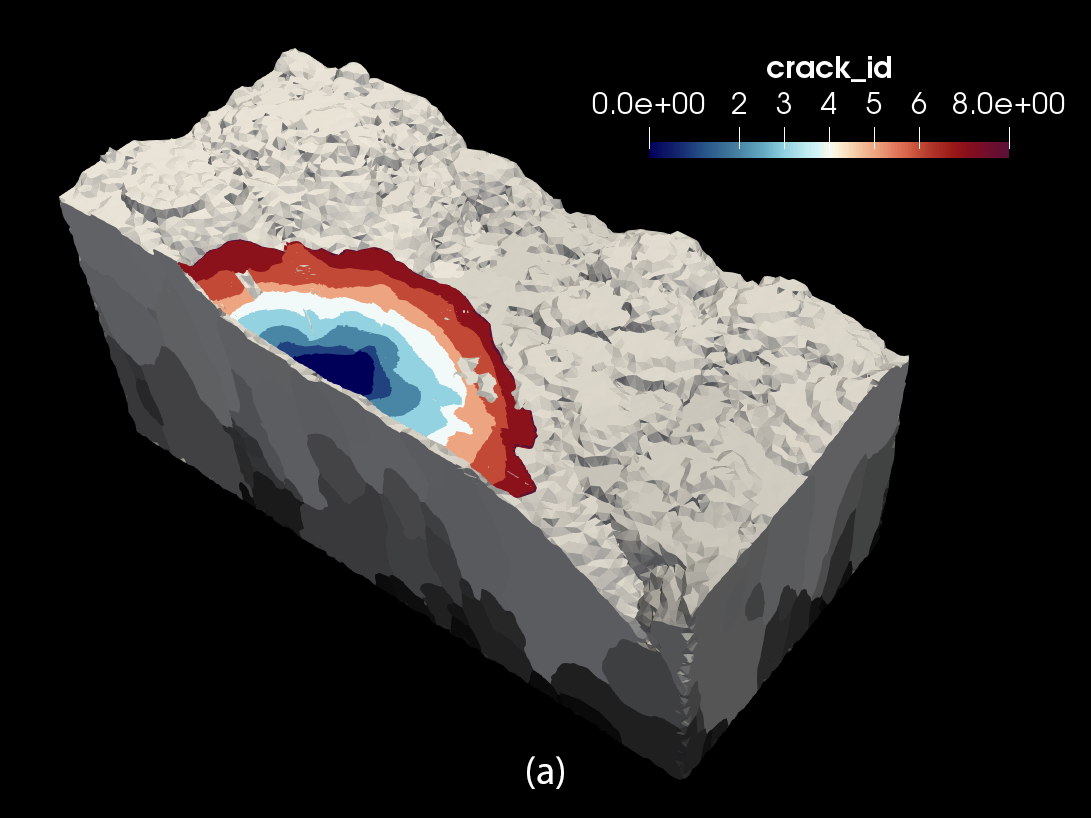
\includegraphics[height=0.25\textwidth]{microstructure_fronts_id}
    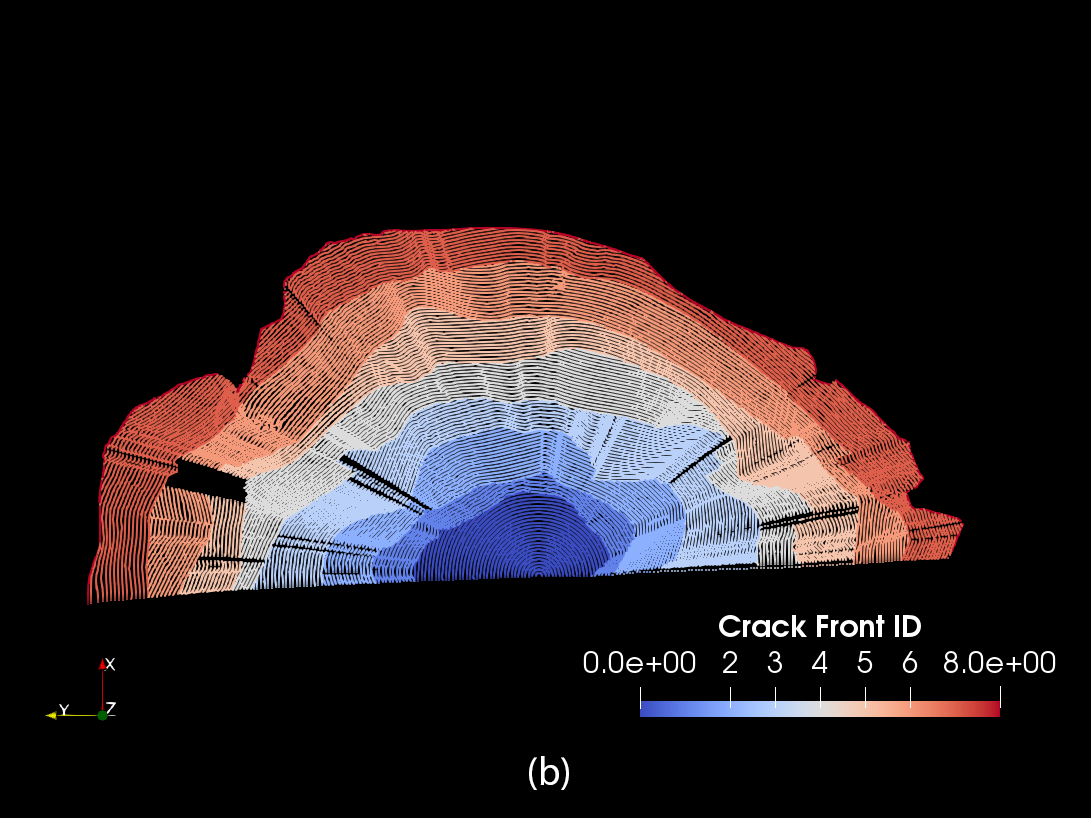
\includegraphics[height=0.25\textwidth]{radial_points_id}
    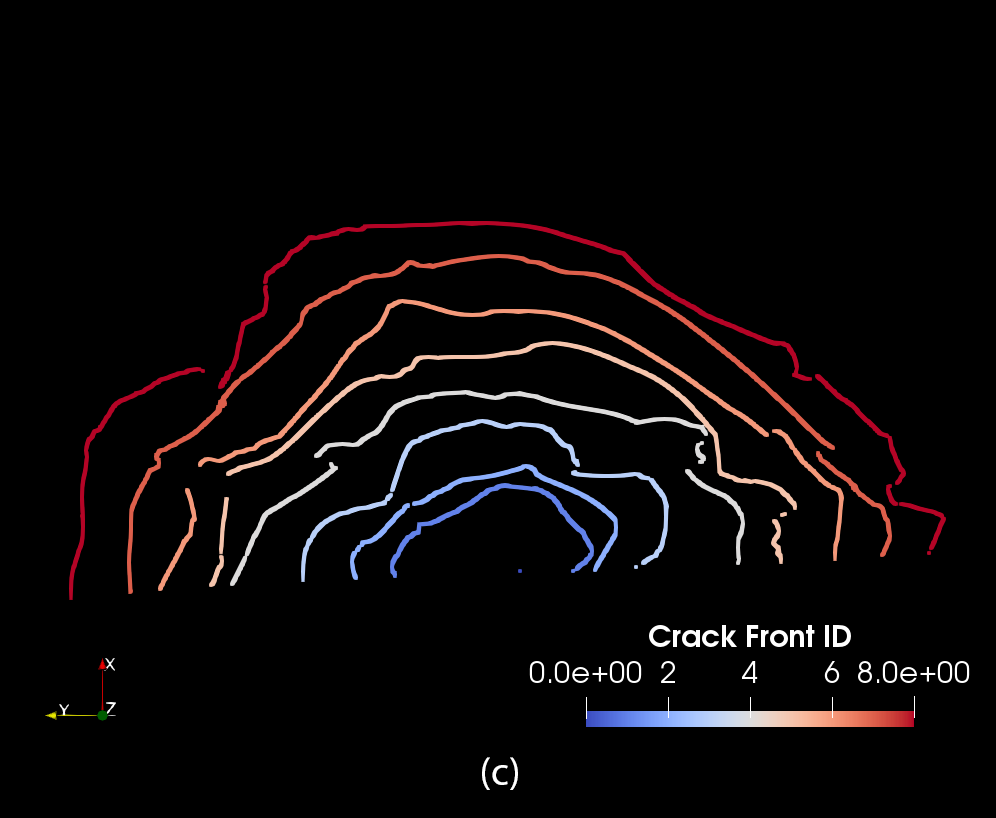
\includegraphics[height=0.25\textwidth]{radial_fronts_id}

    \caption{Microstructure and crack fronts \textbf{(a)}: All crack fronts superimposed on bottom half of microstructure.
             \textbf{(b)}: Crack ID for all points on and between all crack fronts.
             \textbf{(c)}: Crack ID for all points on all crack fronts}
  \label{fig:crack_fronts}
\end{figure}

\begin{table}[p]
  \centering
  \caption{Feature descriptions}
  \label{table:feature-descriptions}
  \begin{tabular}{| p{3cm} | p{11cm} |}
  \hline
  \textbf{Feature} & \textbf{Description} \\
  \hline
  Curvature distance & The difference between
  \begin{enumerate}
    \item the distance from the nucleation point to $x$ and 
    \item the average distance from the nucleation point to the two points 5 $\mu m$ away on either side of this point.
  \end{enumerate} \\ \hline
  Crack normal to nearest grain boundary angle & The angle between the vector normal to the crack front at $x$ and the vector to the nearest grain boundary. \\ \hline
  Distance to average distance & The distance between $x$ and the average distance from the nucleation point for the crack front to which $x$ belongs. \\ \hline
  Distance to grain boundary & Distance from $x$ to the nearest grain boundary. \\ \hline
  Misorientation & The difference between the Euler angles that describe the orientation of the grain in which $x$ resides and those of the nearest grain. \\ \hline
  Previous $\frac{da}{dN}$ & The $\frac{da}{dN}$ of the closest corresponding point on the previous crack front. The closest corresponding point is the one that is closest to the ray extending from the nucleation point to $x$. \\ \hline
  Signed $\Delta$ Taylor factor & The difference in Taylor factor between the grain in which $x$ resides and that of the nearest grain. \\ \hline
  Taylor factor & A number that describes the relationship between the orientation of the grain in which $x$ resides and the direction that the grain is being pulled/stressed. \\ \hline
  \end{tabular}
\end{table}

The goal of the machine learning model was to learn a function of these inputs that best approximated the true unknown function that determined the response variable.  In our case, there were two response variables of interest, $\beta$ and $\frac{da}{dN}$, which could also be called the labels.  These labels are described in Table \ref{table:label-descriptions}.  These values were also calculated for each point $x$ and included in the dataframe.

\begin{table}[b]
  \centering
  \caption{Label descriptions}
  \label{table:label-descriptions}
  \begin{tabular}{| c | p{13cm} |}
  \hline
  \textbf{Label} & \textbf{Description} \\
  \hline
  $\beta$ & An angle describing the change in $z$ for $x$. This is calculated by extending a ray from the nucleation point through $x$, stepping backward along this ray $10 \mu m$ to a point $a$, and stepping forward along this ray $10 \mu m$ to a point $b$. $\beta$ is the angle between the line segment $xa$ and the line segment $xb$. \\ \hline
  $\frac{da}{dN}$ & The distance between $x$ and its closest corresponding point on the next crack front.  The closest corresponding point is the one that is closest to the ray extending from the nucleation point through $x$. \\ \hline
  \end{tabular}
\end{table}

\section{Model training}
The resulting dataframe was loaded into a script written in the R programming language \cite{statistical2009r}.  R was chosen for its rich library of built-in statistical analysis functions, as well as its CARET package \cite{caret2008}, which includes an impressive collection of easy-to-use machine learning algorithms.  The first attempted technique was SVR, using radial basis functions (RBF) as the kernel.  In every case, the data were preprocessed through centering (removing the mean) and scaling (dividing by the standard deviation).  The best values of the hyperparameters $\sigma$ and $C$ were determined using cross-validation over a grid search, i.e., for each $\sigma = 0.1, 0.2, 0.4$ and for each $C = 128, 256, 512$, the best combination was chosen as the one that minimized the cross-validation error metric.  This metric was one of either $RMSE$ or $R^2$, and both are given in the results.  As a first pass, 80\% of the data were used as training data (on which cross-validation was performed) and 20\% was used as testing data.  The data points were split randomly into one of these two sets, and the training data were used to build the model.  For simplicity, only $\frac{da}{dN}$ was used as the response variable, meaning that the predictor would output a single real-valued number.  After the model had been trained on all the training data using the hyperparemeter combination, it was used to predict $\frac{da}{dN}$ for all points in the test set.  These predicted values were compared against the known expected values to calculate the error.  Surprisingly, this initial approach yielded an $R^2$ value of higher than $0.98$, as shown in Table \ref{table:error-metrics}, which appeared to be quite good.  There was, however, a problem with the way in which the data were split.  Since the data points were divided randomly, the test set happened to include many points that were spatially very close to points from the training set.  Thus, the features of these test points highly resembled those of training points, along with similar values of $\frac{da}{dN}$.  These values were much easier to predict, since the model had already seen comparable data points.  The positive result was that this showed the ability of the model to learn complex functions, being able to mimic the expressive power of something like a 1-nearest neighbor classifier.  The negative result was that this splitting approach is not useful for any sort of real-world scenario.  A new approach was needed that better emulated the problem to be solved.

\begin{table}[t]
  \centering
  \caption{Error metrics for all three data splitting strategies of the crack fronts}
  \label{table:error-metrics}
  \begin{tabular}{| c | c | c | c | c | c |} \hline
  \multicolumn{2}{|c|}{Random split} & \multicolumn{2}{|c|}{Leave-one-front-out} & \multicolumn{2}{|c|}{Leave-one-wedge-out} \\ \hline
  $R^2$ & RMSE & $R^2$ & RMSE & $R^2$ & RMSE \\ \hline
  0.984 & 0.000165 & -2.877 & 0.00193 & -2.052 & 0.00159 \\ \hline
  \end{tabular}
\end{table}

\section{Leave-one-front-out (LOFO)}
\index{Cross-Validation ! Leave-one-front-out}
The ideal capability of the model would be to accurately predict future $\frac{da}{dN}$ given some knowledge about how the crack has grown previously, in addition to information about the microstructure.  It would make sense to use this objective as inspiration by training on the earlier crack fronts and testing on the later crack fronts.  The most intuitive strategy would be to use the points from the first $n-1$ crack fronts as training data, and see how well the resulting model predicts the points on the $n^{th}$ crack front.  This meant essentially treating the data as a time-series of crack fronts.  To get the most out of the single dataset, 9 different models were trained, each one leaving out one of the crack fronts during training.  The final test accuracies of all 9 models were averaged together to achieve the mean accuracy.

\section{Leave-one-wedge-out (LOWO)}
\index{Cross-Validation ! Leave-one-wedge-out}
In addition to splitting the data points by the crack front to which they belonged, a different strategy was used that split the data into wedges.  Since the crack began at a single nucleation point and propagated outward radially, its shape was roughly semicircular.  The justification for splitting this shape into wedges was that it provided the model with some points from all crack fronts, giving more context to the expected predictions for $\frac{da}{dN}$.  It also could have some real-world applications, such as handling missing values of measurements for areas with high uncertainty.  The data points were split into 5 wedges of equal angular degree, and 5 models were trained to give a mean test accuracy.

\section{Results}
The resulting values for both error metrics are given in Table \ref{table:error-metrics}.  Also included is Figure \ref{fig:crack_front_prediction}, which includes plots of the crack fronts points, with positions determined using only the actual and predicted values of $\frac{da}{dN}$, i.e. flattening the crack fronts for visualization.

\begin{figure}[b]
  \centering
  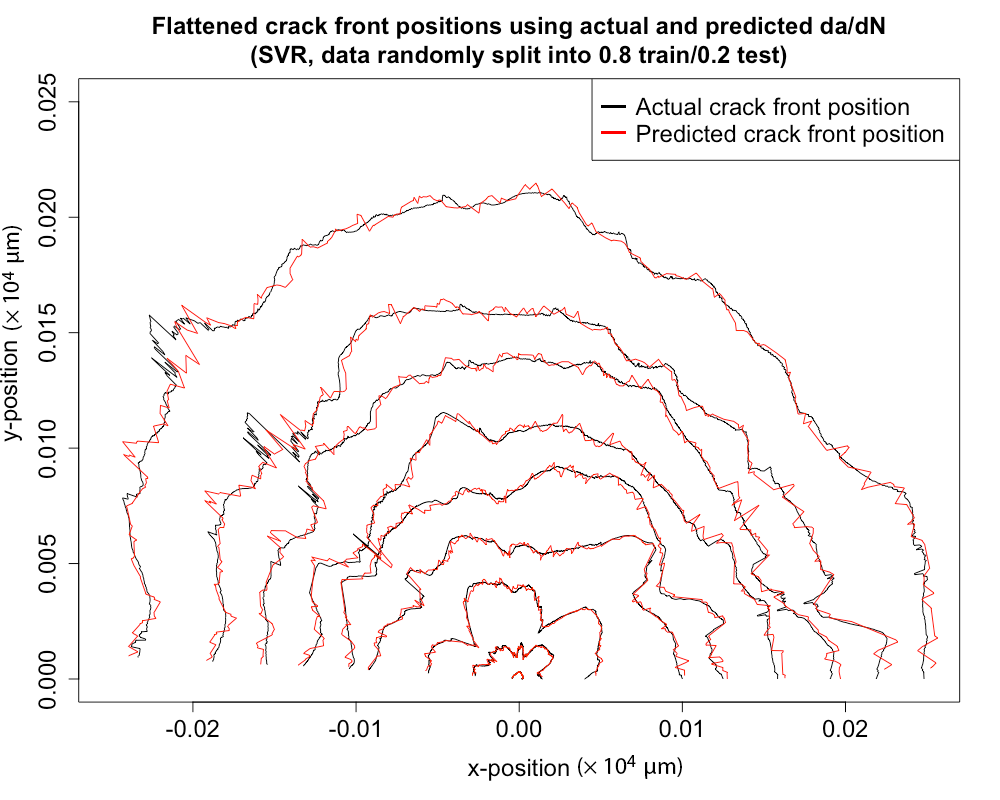
\includegraphics[width=0.475\textwidth]{random_split}
  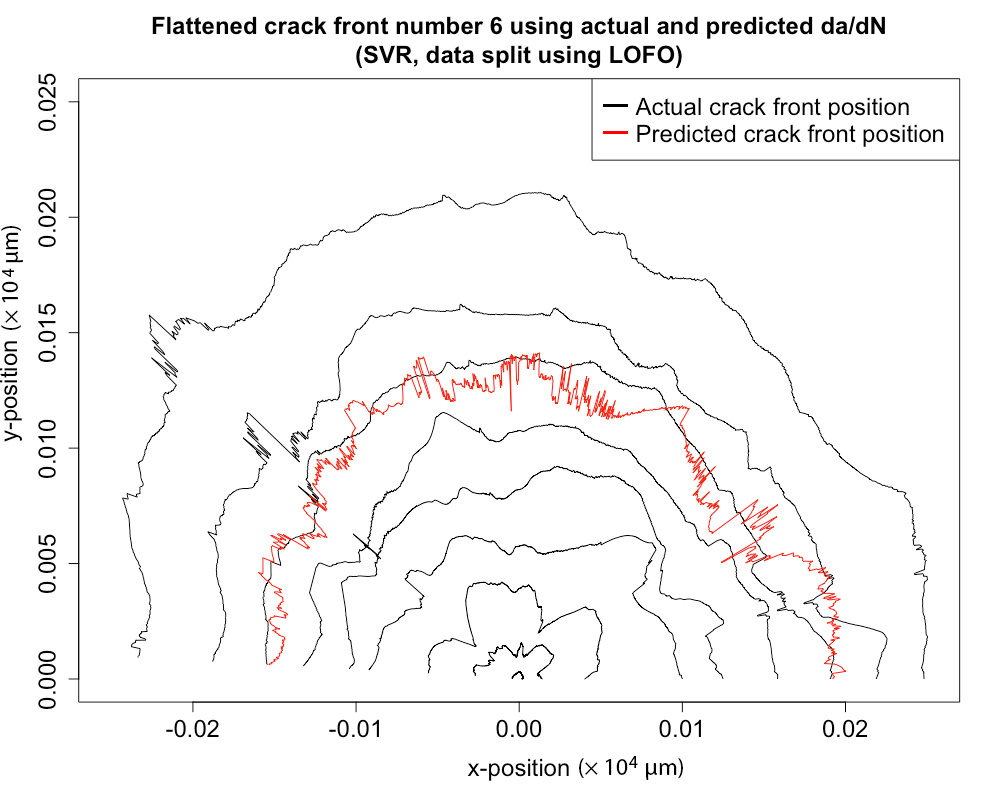
\includegraphics[width=0.475\textwidth]{time_split}

  \caption{Projected crack-front positions based on average crack-growth rates applied over 10,000-cycle intervals.
           \textbf{Left}: visualization of the predicted crack fronts using a random split of training
and testing data.
           \textbf{Right}: visualization of the predicted 6th crack front using a LOFO split of training and testing data.}
  \label{fig:crack_front_prediction}
\end{figure}

\section{Conclusion}
It is clear that there is not enough predictive power in these 7 features alone to give accurate predictions of the crack growth rate, especially for such a small amount of data.  Although growth-rate data are confined to these 9 crack fronts, it would be ideal to leverage more of the available data from this single experiment.  Furthermore, feature selection, which was based on prior domain knowledge, could be improved.  A model that could learn the relevant features given a relatively raw representation of the data might perform better than one that uses hand-picked features.  The next two chapters focus on discovering this representation and using it effectively in an appropriate machine learning model.

\bibliographystyle{ieeetr}
\bibliography{\jobname}
